%--------------------------------------------------------------------------------------------------
\begin{frame}[t]
    \frametitle{Image Recognition Models}
    \framesubtitle{An ongoing revolution since 2012}
    \small
    \begin{center}
        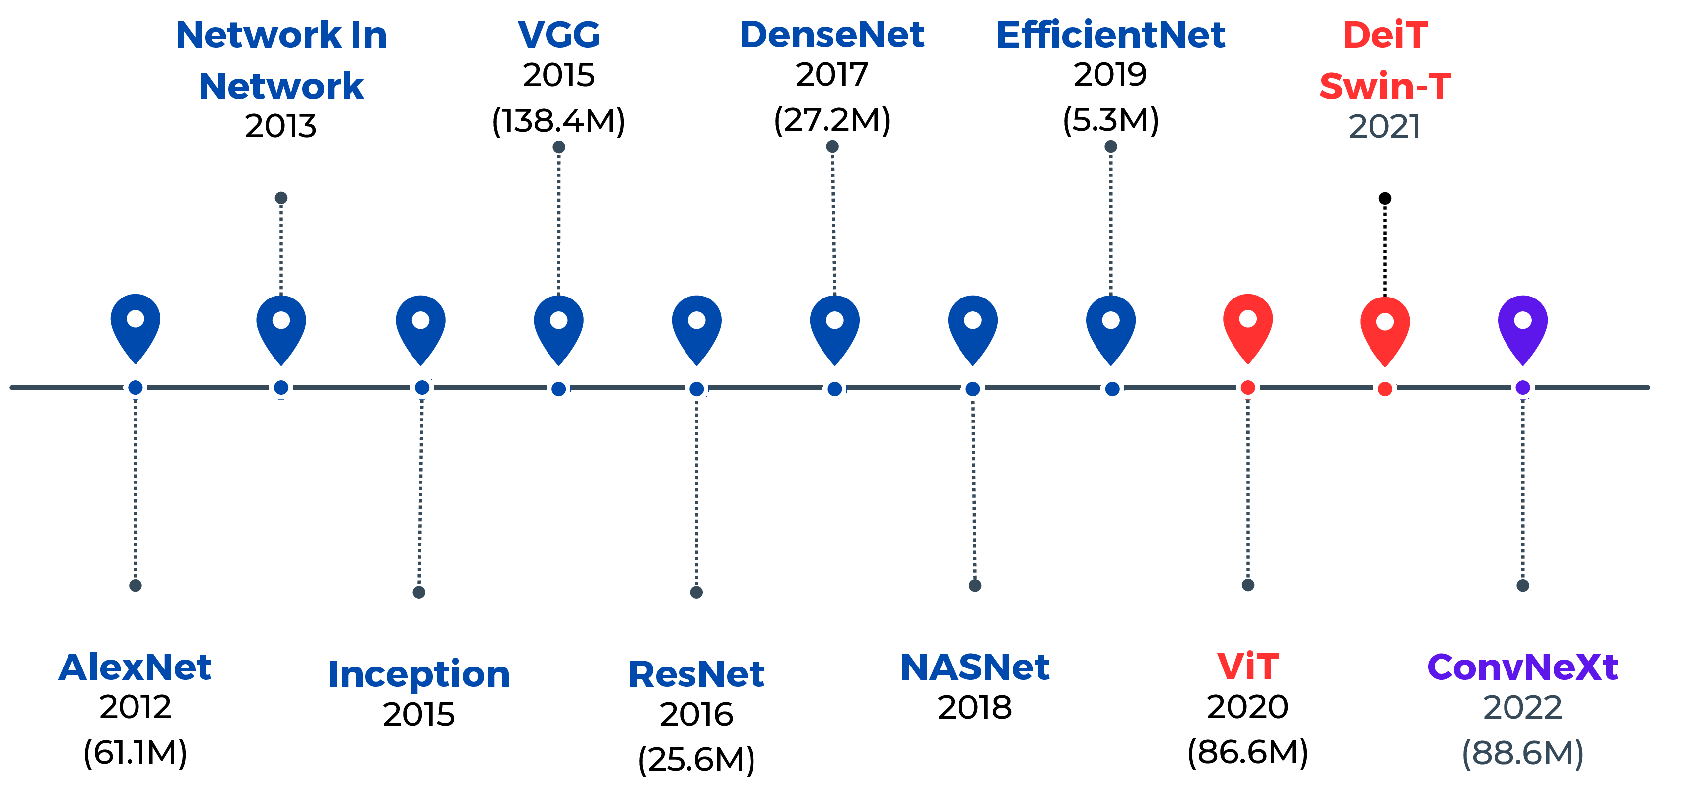
\includegraphics[width=.8\textwidth]{fig/intro/comp_cv_ai/img/imrecon_timeline.pdf}    
    \end{center}
    \vspace{-10pt}
    \pause
    \begin{columns}
        \column[T]{.5\textwidth}
            Contributing factors:
            \begin{itemize}
                \item Widespread of Internet.
                \item Big Dataset collection.
                \item Popularization of the GPU.
            \end{itemize}
        \pause
        \column[T]{.5\textwidth}
        Two paradigms:\\
            \blue{Convolutional Neural Networks (CNNs).}\\
            \red{Transformers.}
    \end{columns}
\end{frame} 
%--------------------------------------------------------------------------------------------------
\subsection*{xAI}
\begin{frame}[t]
    \frametitle{Interpretability}
    \framesubtitle{Motivation}
    \small
    We are interested in understanding models,\\
    behaving like a black box:\\\vspace{-10pt}
    \begin{center}
            %\begin{center}
    \begin{tikzpicture}[] 
        %% Anchors
        \node[rectangle, opacity=.75, draw=black, fill=black!, minimum width=5cm, minimum height=2.5cm]
            at (0,0) (blackbox) {};
        \node[] at (-4, 0) (in) {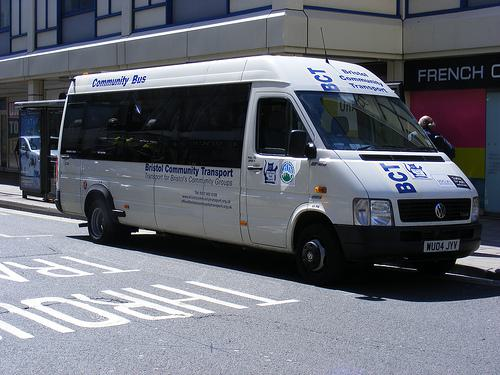
\includegraphics[scale=0.2]{fig/castream/img/Comparable/figure1/original/27079.jpeg}};
        \node[] at (4, 0) (out) {\emph{Car ID}\\\emph{427}};
        %% Tags
        \node[] at (in.north) (intxt) {$x$};
        \node[] at (0, 1.5) (bboxtxt) {$f$};
        \node[] at (4, 1.1) (pred) {$y$};
        %% Arrows
        \draw[->] (in) -- (blackbox);
        \draw[->] (blackbox) -- (out);

\end{tikzpicture}    
\end{center}

            \begin{center}
    \begin{tikzpicture}[] 
        %% Anchors
        \node[rectangle, opacity=.75, draw=black, fill=black!, minimum width=5cm, minimum height=2.5cm]
            at (0,0) (blackbox) {};
        \node[] at (-4, 0) (in) {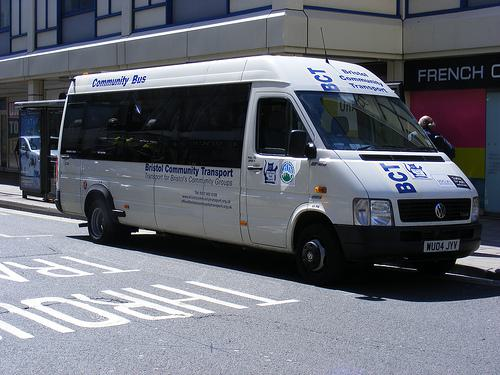
\includegraphics[scale=0.2]{fig/castream/img/Comparable/figure1/original/27079.jpeg}};
        \node[] at (4, 0) (out) {\emph{Car ID}\\\emph{427}};
        %% Tags
        \node[] at (in.north) (intxt) {$x$};
        \node[] at (0, 1.5) (bboxtxt) {$f$};
        \node[] at (4, 1.1) (pred) {$y$};
        %% Arrows
        \draw[->] (in) -- (blackbox);
        \draw[->] (blackbox) -- (out);

\end{tikzpicture}    
\end{center}

        \textbf{We want to \emph{know why} $f(x)\rightarrow y$}\\
    \end{center}
    %\pause
    %\vspace{-20pt}
    %\pause
    %\begin{center}
    \begin{tikzpicture}[] 
        \node[] at (-4, 0) (cam) {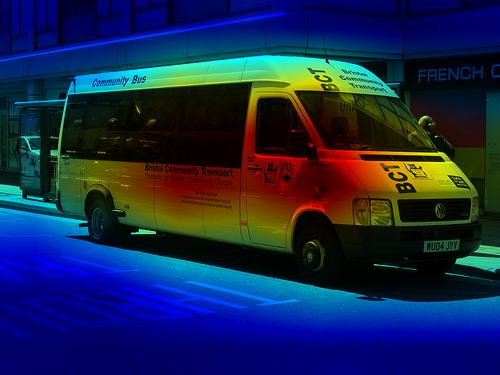
\includegraphics[width=.33\textwidth]{fig/castream/img/Comparable/figure1/gradcam/27079}};
        \node[] at (-4, 1.5) (camtxt) {\scriptsize Saliency Maps};
        \pause
        \node[] at (0, 0) (grad) {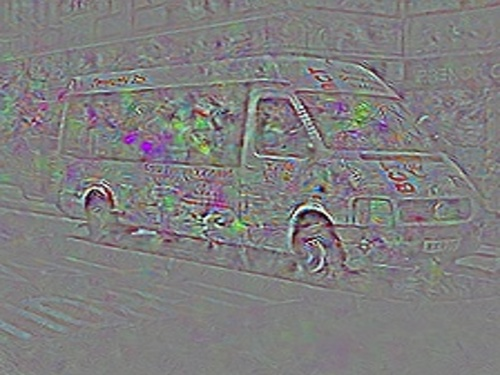
\includegraphics[width=.33\textwidth]{fig/intro/comp_cv_ai/img/gb_van}};
        \node[] at (0, 1.5) (gradtxt) {\scriptsize Gradients};
        \pause
        \node[] at (3.5, .5) (wshld) {
\includegraphics[scale=.125]{fig/intro/comp_cv_ai/img/parts_van/wshld.png}};
        \node[] at (4, 1.5) (other) {\scriptsize Other Representations};
        \node[] at (wshld.south east) (lights) {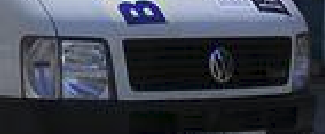
\includegraphics[scale=.125]{fig/intro/comp_cv_ai/img/parts_van/lights.png}};
        \node[] at (lights.south west) (front) {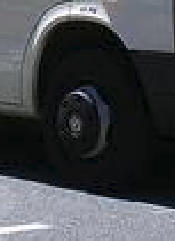
\includegraphics[scale=.125]{fig/intro/comp_cv_ai/img/parts_van/front.png}};
        \node[] at (front.west) {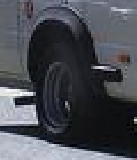
\includegraphics[scale=.125]{fig/intro/comp_cv_ai/img/parts_van/rear.png}};
        \pause
        \node[rectangle, opacity=1, draw=red, minimum width=8cm, minimum height=2.75cm, very thick] at (-2, 0) (rect_chosen) {};
        \node at (-1.5, -1.75) {\scriptsize We demonstrate improvements in these approaches};
    \end{tikzpicture}    
\end{center}

\end{frame}
%--------------------------------------------------------------------------------------------------